\section{TP4 Separate user identity, sign-up and self-care from product dependencies}
\label{sec:principle-tp4-seperate-user-identity}

Die meisten Dienste im Internet verlangen heute nach der Erstellung eines Benutzerkontos. Ein Forum lässt bspw. das Verfassen von Beiträgen erst zu, nachdem sich der potentielle Autor mit seiner E-Mail-Adresse, einem Benutzernamen und einem Passwort erfolgreich registriert hat. Zur Praxis gehört zudem, dass der Benutzer seine Angaben mittels einem eindeutigen Link, welcher ihm per E-Mail zugestellt wird, bestätigt.

Eine solche Registrierung hat für den Benutzer eines Dienstes als auch für den Betreiber dessen auf den ersten Blick hauptsächlich Vorteile:

\begin{itemize}
	\item Die User Experience kann von Anfang bis Ende auf den Benutzer zugeschnitten und optimiert werden. (Beispiele: Speichern der eigenen Zeitzone für korrekte Datums- und Zeitangaben, Personalisierung der Frontseite usw.)
	\item Sicherstellung der Identität: Jedes Benutzerkonto resp. jeder Benutzername wird immer von der selben Person verwendet
	\item Durch gezielte Auswertungen kann der Betreiber sein Angebot optimieren und ggf. Marketing betreiben resp. Werbung in seinem Dienst schalten
\end{itemize}

Bei genauerer Analyse ergeben sich aber auch nicht zu vernachlässigende negative Faktoren:

\begin{itemize}
	\item Der Benutzer muss bei jedem neuen Dienst wiederholt ein Konto erstellen und so erneut persönlichen Informationen preisgeben
	\item Der Betreiber muss sich um die Speicherung und Sicherheit der Benutzerinformationen kümmern
	\item Der Mechanismus zur Identitätsüberprüfung muss vom Betreiber selber umgesetzt werden
	\item Nach einer gewissen Zeit hat ein Benutzer tendenziell keine Kontrolle mehr darüber, wo er sich registriert und seine Informationen hinterlegt hat
	\item Die Umsetzung von Zugriffskontrollen (Wer darf welche Informationen eines Benutzers sehen etc.) ist mit entsprechenden Aufwänden verbunden
\end{itemize}

Vorangegangene Auflistungen sind exemplarisch und nicht abschliessend, gewähren aber einen guten Einblick die Thematik.
\newline\newline
Tilkovs \emph{TP4} schlägt nun die Separierung von Benutzerinformationen und der eigentlichen Registrierung bei einem Dienst vor.

Der Vorreiter OpenID \cite{OpenID} und insbesondere die omnipräsenten sozialen Netzwerke erleichtern eben diese Auftrennung Heute mehr den je.
\newline\newline
Ein Konto bei Facebook oder Twitter ermöglicht so den Zugriff auf Dienste Dritter: Möchte ein Benutzer personalisierte News bei \emph{20 Minuten} lesen, kann er sich mit seinem Facebook Konto anmelden \cite{20min} ohne genauere Informationen zu seiner Person wiederholt angeben zu müssen. Dabei kann er zudem gezielt steuern, welche Informationen an den Dienstbetreiber durch Facebook weitergegeben werden oder nicht.
\newline\newline
Abbildung \ref{fig:applicationdata-vs-identityprovider} visualisiert das Konzept der getrennten Datenhaltung im Bezug auf Applikations- und Identitätsspezifsche Informationen.

\begin{figure}[H]
	\centering
	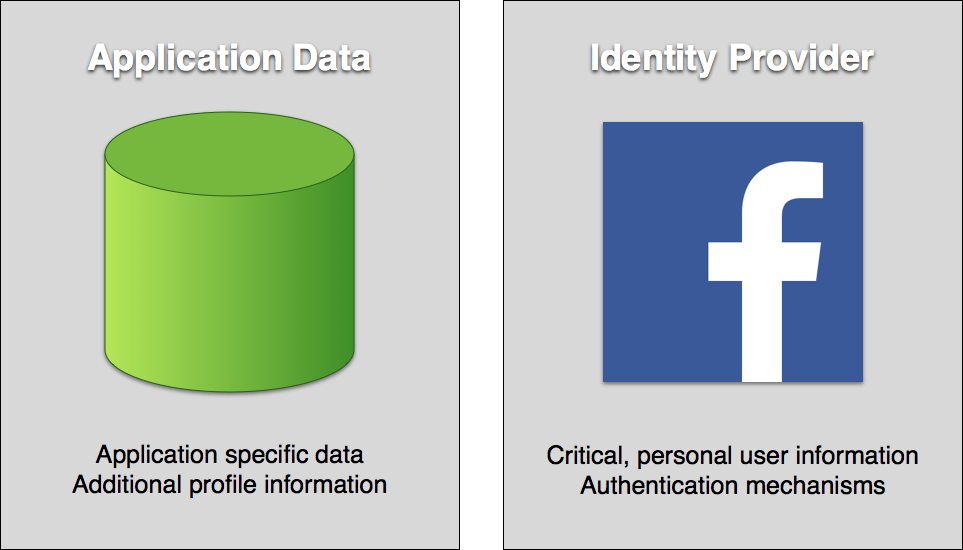
\includegraphics[width=9cm]{content/principle-demonstration/images/applicationdata-vs-identityprovider.png}
	\caption{Separierung der Applikations- und Identitätsinformationen}
	\label{fig:applicationdata-vs-identityprovider}
\end{figure}

In der Abbildung \ref{fig:applicationdata-vs-identityprovider} ist zudem ersichtlich dass ein \emph{Identity Provider} meist auch den Mechanismus zur effektiven Authentisierung des Benutzers bereitstellt. Viele Anbieter setzen hier auf den de facto Standard \emph{OAuth} \cite{oauth} oder verwenden eigene Implementationen.


\subsection*{Geplante Umsetzung}

Für die Beispielapplikation \emph{Roomies} hat das Projektteam geplant, Facebook als hauptsächlichen und einzigen \emph{Identity Provider} zu einzusetzen. Dabei soll das offizielle \emph{Facebook Login for Web} \cite{facebooklogin} \gls{SDK} eingesetzt werden.

Innerhalb der Beispielapplikation soll lediglich die Facebook ID sowie der Name des Benutzers persistent gespeichert werden. Alle anderen Informationen sollen bei Facebook verbleiben resp. gar nicht erst auf diese zugegriffen werden.


\subsection*{Konkrete Umsetzung}

Für die tatsächliche Anbindung des \emph{Facebook Login for Web} \cite{facebooklogin} \gls{SDK}'s wurde wie im Abschnitt \ref{sec:sad-layers} ``\nameref{sec:sad-layers}'' des Kapitels ``\nameref{sec:sad}'' beschrieben die quelloffene Bibliothek \emph{Passport} \cite{Passportjs} verwendet.




\subsection*{Diskussion}
